
\documentclass[12pt, a4paper, oneside, chapter=TITLE, section=TITLE, english, brazilian]{abntex2}

% Arquivo com a formatação é lido aqui. Não deve ser modificado

% Arquivo com a formatação do TCC. Este arquivo não deve ser modificado.
\usepackage[utf8]{inputenc}
\usepackage[T1]{fontenc}
\usepackage{amsmath}
\usepackage{amssymb,amsfonts,textcomp}
\usepackage{color}
\usepackage{array}
\usepackage{supertabular}
\usepackage{listings}    % Para as linguagens de programação
\usepackage{lastpage}		 % Usado pela Ficha catalográfica
\usepackage{indentfirst} % Indenta o primeiro parágrafo de cada seção.
\usepackage{hhline}
\usepackage{hyperref}
\usepackage[pdftex]{graphicx}
\graphicspath{ {./figuras/} }

\newcolumntype{Y}{>{\centering\arraybackslash}X}   % Colunas centralizadas
\newcolumntype{L}{>{\raggedright\arraybackslash}X} % Coluna 'L' que é um 'X' alinhado à esquerda

% Retira as mensagens de aviso do pacote Glossaries
\let\printglossary\relax
\let\theglossary\relax
\let\endtheglossary\relax

% Coloca Seções em maiúsculas sem negrito no Sumário
\makeatletter
\let\oldcontentsline\contentsline
\def\contentsline#1#2{%
  \expandafter\ifx\csname l@#1\endcsname\l@section
    \expandafter\@firstoftwo
  \else
    \expandafter\@secondoftwo
  \fi
  {%
    \oldcontentsline{#1}{\normalfont\MakeTextUppercase{#2}}%
  }{%
    \oldcontentsline{#1}{#2}%
  }%
}
\makeatother

% Pacote glossaries
\usepackage[subentrycounter,seeautonumberlist,nonumberlist=true]{glossaries}

% Citações de referências no formato alfabético e negrito
\usepackage[alf, abnt-emphasize=bf]{abntex2cite}

% Margens definidas como 3cm acima e à esquerda, e 2cm abaixo e à direita
\usepackage[left=30mm, top=30mm, right=20mm, bottom=20mm]{geometry}

% Definições das macros utilizadas no TCC

% Definições das macros utilizadas no TCC (modifique esse arquivo)

\instituicao{
  UNIVERSIDADE FEDERAL DO RIO DE JANEIRO \par
  INSTITUTO DE COMPUTAÇÃO \par
  CURSO DE BACHARELADO EM CIÊNCIA DA COMPUTAÇÃO
}

\title{MODELO DE MONOGRAFIA DE TRABALHO DE CONCLUSÃO DE CURSO: \\ Modelo em Latex}

\autor{Nome Completo do Aluno 1 \\ Nome Completo do Aluno 2}

\orientador{Prof. João José da Silva}

\coorientador{Profa. Maria da Penha}

\local{RIO DE JANEIRO}

\data{\the\year}

\preambulo{Trabalho de conclusão de curso de graduação apresentado ao Instituto de Computação da Universidade Federal do Rio de Janeiro como parte dos requisitos para obtenção do grau de Bacharel em Ciência da Computação.}


\setlength{\cftbeforechapterskip}{0pt}

% Para corrigir algumas fontes e estilos
\renewcommand{\ABNTEXchapterfont}{\bfseries \rmfamily}  % Capítulos em Bold e Maiúsculas
\renewcommand{\ABNTEXchapterfontsize}{\normalsize}
\renewcommand{\ABNTEXsectionfont}{\rmfamily}            % Seções em  Maiúsculas apenas
\renewcommand{\ABNTEXsectionfontsize}{\normalsize}
\renewcommand{\ABNTEXsubsectionfont}{\bfseries}         % Subseções em Bold apenas
\renewcommand{\ABNTEXsubsectionfontsize}{\normalsize}
\renewcommand{\lstlistingname}{Código}                  % Nome para os códigos no texto
\renewcommand{\lstlistlistingname}{Lista de \lstlistingname s}

% Redefine formato da lista
\makeatletter
\renewcommand{\l@lstlisting}[2]{%
  \begingroup
  \normalfont
    \let\oldnumberline\numberline
    \renewcommand{\numberline}[1]{\lstlistingname\space##1~  --~  }%
    \@dottedtocline{1}{0em}{2.3em}{#1}{#2}%
  \endgroup
}
\makeatother

% Para retirar < e > da URL nas referências.
\usepackage{url6023}

% Cria quadros com numeração
\newcommand{\quadroname}{Quadro}
\newcommand{\listofquadrosname}{Lista de quadros}
\newfloat[chapter]{quadro}{loq}{\quadroname}
\newlistof{listofquadros}{loq}{\listofquadrosname}
\newlistentry{quadro}{loq}{0}
\setfloatadjustment{quadro}{\centering}
\counterwithout{quadro}{chapter}
\renewcommand{\cftquadroname}{\quadroname\space}
\renewcommand*{\cftquadroaftersnum}{\hfill--\hfill}
\setfloatlocations{quadro}{hbtp}
\makeatletter
\newcommand\arraybslash{\let\\\@arraycr}
\makeatother

% Redefine a macro para imprimir a capa
\renewcommand{\imprimircapa}{%
  \begin{capa}%
    \center
    \imprimirinstituicao
    \par
    \vspace*{1cm}
    \MakeUppercase{\imprimirautor}
    \vfill
    \begin{center}
      \imprimirtitulo
    \end{center}
    \vfill
    \imprimirlocal
    \par
    \imprimirdata
    \vspace*{1cm}
  \end{capa}
}

% Redefine a macro para imprimir a folho de rosto
\renewcommand{\imprimirfolhaderosto}{%
  \begin{capa}%
    \center
    \par
    \vspace*{1cm}
    \MakeUppercase{\imprimirautor}
    \vfill
    \begin{center}
      \imprimirtitulo
    \end{center}
    \vfill
    \hspace*{\fill}\parbox[b]{.5\textwidth}{%
      \linespread{1}\selectfont
      \imprimirpreambulo
    }
    \vfill
    \flushright
    Orientador: \imprimirorientador\\

    Co-orientador: \imprimircoorientador\\
    \vfill
    \begin{center}
      \large\imprimirlocal
      \par
      \large\imprimirdata
      \vspace*{1cm}
    \end{center}
  \end{capa}
}

% Informações do PDF inseridas automaticamente
% Atualizar apenas as palavras-chave se necessário
% Não modificar as cores dos links e referências
\makeatletter
\hypersetup{
  pdftitle    = {\@title},
  pdfauthor   = {\@author},
  pdfsubject  = {\imprimirpreambulo},
  pdfkeywords = {MONOGRAFIA}{CIÊNCIA DA COMPUTAÇÃO}{DCC-UFRJ},
  pdfcreator  = {LaTeX with abnTeX2},
  colorlinks  = true,
  linkcolor   = black,
  citecolor   = black,
  urlcolor    = black
}
\makeatother

% Definição de cores para linguagens de programação
\definecolor{dkgreen}{rgb}{0,0.6,0}
\definecolor{gray}{rgb}{0.5,0.5,0.5}
\definecolor{purple}{rgb}{0.8,0,0.3}
\definecolor{orange}{rgb}{1,0.4,0}
\definecolor{lightlightgray}{rgb}{.95,.95,.95}
\definecolor{lightgray}{rgb}{.9,.9,.9}
\definecolor{lightgray2}{rgb}{.85,.85,.85}
\definecolor{darkgray}{rgb}{.4,.4,.4}

% Comando para inserir a listagem de código, tem 4
% parâmetros: Linguagem, Caption, Label, Nome do Arquivo
\newcommand{\includecode}[4][C]{\mbox{\lstinputlisting[caption=#2, label=#3, escapechar=, style=custom#1]{#4}}}

% Define características em comum e numeração sequencial
\lstset{numberbychapter=false, framexleftmargin=5mm, frame=shadowbox, rulesepcolor=\color{gray}}

% Redefine o ambiente 'siglas' para alinhar como o índice remissivo
\renewenvironment{siglas}{
  \pretextualchapter{\listadesiglasname} % Título e formatação padrão do abntex2
  \begin{list}{}{
    \setlength{\labelwidth}{2.5cm} % Largura da coluna das siglas
    \setlength{\leftmargin}{\labelwidth + 0cm} % Margem esquerda + espaçamento
    \setlength{\labelsep}{0cm} % Espaço entre sigla e texto
    \setlength{\itemsep}{0pt} % Espaçamento entre itens
    \setlength{\parsep}{0pt} %
    \renewcommand{\makelabel}[1]{##1 \hfill}%
  }
}{
  \end{list}
}

% Redefine o ambiente 'simbolos' para alinhar como o índice remissivo
\renewenvironment{simbolos}{
  \pretextualchapter{\listadesimbolosname} % Título e formatação padrão do abntex2
  \begin{list}{}{
    \setlength{\labelwidth}{2.5cm} % Largura da coluna das siglas
    \setlength{\leftmargin}{\labelwidth + 0cm} % Margem esquerda + espaçamento
    \setlength{\labelsep}{0cm} % Espaço entre sigla e texto
    \setlength{\itemsep}{0pt} % Espaçamento entre itens
    \setlength{\parsep}{0pt}
    \renewcommand{\makelabel}[1]{##1 \hfill}
  }
}{
  \end{list}
  \cleardoublepage % Força nova página, respeitando estilos de capítulos
}

% A leitura da formatação das linguagens é feita aqui.

% Aqui você pode personalizar a linguagem C
\lstdefinestyle{customC}{
  language         = C,
  breaklines       = true,
  basicstyle       = \footnotesize\ttfamily,
  keywordstyle     = \bfseries\color{blue},
  commentstyle     = \itshape\color{purple},
  identifierstyle  = \color{black},
  stringstyle      = \color{orange},
  showstringspaces = false
}

% Aqui você pode personalizar a linguagem Java
\lstdefinestyle{customJava}{
  language         = Java,
  breaklines       = true,
  basicstyle       = \footnotesize\ttfamily,
  keywordstyle     = \bfseries\color{blue},
  commentstyle     = \itshape\color{purple},
  identifierstyle  = \color{black},
  stringstyle      = \color{orange},
  showstringspaces = false
}

% Aqui você pode personalizar a linguagem C++
\lstdefinestyle{customC++}{
  language         = C++,
  breaklines       = true,
  basicstyle       = \footnotesize\ttfamily,
  keywordstyle     = \bfseries\color{blue},
  commentstyle     = \itshape\color{purple},
  identifierstyle  = \color{black},
  stringstyle      = \color{orange},
  showstringspaces = false
}

% Aqui você pode personalizar a linguagem Javascript
\lstdefinestyle{customJavaScript}{
  language         = JavaScript,
  breaklines       = true,
  basicstyle       = \footnotesize\ttfamily,
  keywordstyle     = \bfseries\color{blue},
  commentstyle     = \itshape\color{purple},
  identifierstyle  = \color{black},
  stringstyle      = \color{orange},
  showstringspaces = false
}

% Javascript
\lstdefinelanguage{JavaScript}{
  aboveskip       = 15pt,
  keywords        = {typeof, new, true, false, catch, function, return, null, catch, switch, var, if, in, while, do, else, case, break},
  keywordstyle    = \color{blue}\bfseries,
  ndkeywords      = {class, export, boolean, throw, implements, import, this},
  ndkeywordstyle  = \color{darkgray}\bfseries,
  identifierstyle = \color{black},
  sensitive       = false,
  comment         = [l]{//},
  morecomment     = [s]{/*}{*/},
  commentstyle    = \color{purple}\ttfamily,
  stringstyle     = \color{red}\ttfamily,
  morestring      = [b]',
  morestring      = [b]",
  rulecolor       = \color{lightgray2},
  breaklines      = true,
  basicstyle      = \footnotesize\ttfamily,
  frame           = single,
  backgroundcolor = \color{lightlightgray}
}

% Aqui você pode personalizar o formato JSON
\lstdefinestyle{customJSON}{
  language         = JSON,
  breaklines       = true,
  basicstyle       = \footnotesize\ttfamily,
  keywordstyle     = \bfseries\color{blue},
  commentstyle     = \itshape\color{purple},
  identifierstyle  = \color{black},
  stringstyle      = \color{orange},
  showstringspaces = false
}

% JSON
\lstdefinelanguage{JSON}{
  aboveskip       = 15pt,
  string          = [s]{"}{"},
  stringstyle     = \color{blue},
  comment         = [l]{:},
  commentstyle    = \color{black},
  rulecolor       = \color{lightgray2},
  breaklines      = true,
  basicstyle      = \footnotesize\ttfamily,
  frame           = single,
  backgroundcolor = \color{lightlightgray}
}

% Aqui você pode personalizar a linguagem de montagem do SAPIENS
\lstdefinestyle{customSapiens}{
  language         = Sapiens,
  breaklines       = true,
  basicstyle       = \footnotesize\ttfamily,
  keywordstyle     = \bfseries\color{blue},
  commentstyle     = \itshape\color{purple},
  identifierstyle  = \color{black},
  stringstyle      = \color{orange},
  showstringspaces = false
}

% Linguagem de Montagem
\lstdefinelanguage{Sapiens}{
  aboveskip       = 15pt,
  keywordstyle    = \color{blue}\bfseries,
  comment         = [l]{;},
  commentstyle    = \color{purple},
  rulecolor       = \color{lightgray2},
  breaklines      = true,
  basicstyle      = \footnotesize\ttfamily,
  frame           = single,
  backgroundcolor = \color{lightlightgray},
  language        = [x86masm]Assembler,
  morekeywords    = {DB, DS, DW, JN, JSR, LDA, ORG, STA, STS, TRAP}
}



% Comando para inicializar o glossário
\makeglossaries

% Entradas do glossário

\newglossaryentry{equilibrio}{
  name        = {Equilíbrio da configuração},
  see         = [veja também]{componente},
  description = {Consistência entre os \glspl{componente}}
}

\newglossaryentry{latex}{
  name        = {LaTeX},
  description = {Ferramenta de computador para autoria de documentos criada por L. Lamport}
}

\newglossaryentry{abntex2}{
  name        = {abnTeX2},
  see         = {latex},
  description = {Suíte para LaTeX que atende os requisitos das normas da ABNT para elaboração de documentos técnicos e científicos brasileiros}
}

\newglossaryentry{maths}{
  name        = {Matemática},
  description = {Matemática é o que os matemáticos fazem}
}

\newglossaryentry{formula}{
  name        = {Fórmula},
  description = {Uma expressão matemática}
}

\newacronym{mdc}{MDC}{Máximo Divisor Comum}

\newacronym{mmc}{MMC}{Mínimo Múltiplo Comum}


\begin{document}
  \pretextual

  % Capa (obrigatório)
  \setcounter{page}{1}
  \imprimircapa

  % Folha de Rosto (obrigatório)
  \imprimirfolhaderosto

  % Ficha catalográfica (obrigatório)
  % Para elaborar a ficha catalográfica siga as instruções em https://fichacatalografica.sibi.ufrj.br/
  \vspace*{1cm}
  \begin{fichacatalografica}
    \begin{figure}[b]
      \centering
      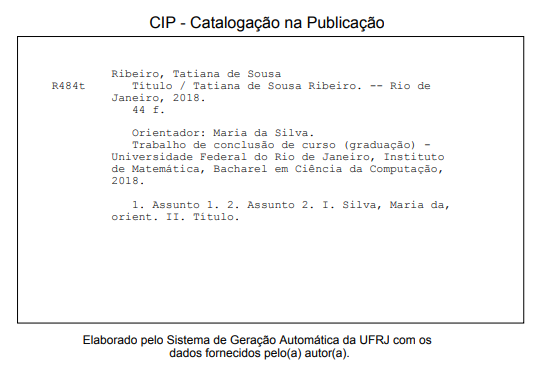
\includegraphics[width=14.217cm,height=9.929cm]{ModeloMonografiaDCCUFRJ-img001.png}
    \end{figure}
    % Opcionalmente você pode usar \includepdf{fig_ficha_catalografica.pdf}
  \end{fichacatalografica}
  \vspace*{1cm}

  {\centering\color{red}\textrm{Nota: Não entrar com o título do trabalho na ficha catalográfica em caixa alta.}}

  % Folha de Aprovação (obrigatório)
  % Substitua todo o conteúdo desta página por uma
  % imagem da página assinada pela banca com o comando abaixo:
  % \includepdf{folhadeaprovacao_final.pdf}
  \begin{folhadeaprovacao}
\vspace*{\fill}
\begin{center}
    {\MakeUppercase{\imprimirautor}}
    \vspace*{\fill}
    \begin{center}
      \imprimirtitulo \\
    \end{center}
    \vspace*{\fill}
  \end{center}
  \hspace*{\fill}\parbox[b]{.5\textwidth}{%
    \linespread{1}\selectfont
    \imprimirpreambulo
}

\vspace*{\fill}
    \begin{flushleft}
 % Alterar a data ou preencher à mão
   Aprovado em \_\_\_ de \_\_\_\_\_\_\_\_\_\_\_\_\_\_ de \_\_\_\_\_\_\_
  \par
  \vspace*{\fill}

BANCA EXAMINADORA:
\end{flushleft}

  \vspace*{\fill}
   \assinatura{Nome do Professor Orientador \\ Titulação (Instituição)}
   \vspace*{\onelineskip}
   \assinatura{Nome do Professor1 \\ Titulação (Instituição)}
   \vspace*{\onelineskip}
   \assinatura{Nome do Professor2\\ Titulação (Instituição)}
   %\assinatura{Nome do Professor, Titulação (Instituição)}
   %\assinatura{Nome do Professor, Titulação (Instituição)}
\vspace*{\fill}
\end{folhadeaprovacao}


  % Dedicatória (opcional)
  
\begin{dedicatoria}

  \clearpage

  % Este comando empurra todo o conteúdo que vem depois dele para a parte inferior da página.
  \vspace*{\fill}

  \hfill
  \begin{minipage}{0.5\textwidth}
    % O uso de \textit{} (itálico) é opcional, mas comum para dedicatórias.
    \raggedleft
    \textit{Dedicatória: Texto no qual o autor do trabalho oferece homenagem ou dedica o seu trabalho a alguém. Recomenda-se que o texto da dedicatória seja breve.} \\
    \textit{Deve ser começar na metade de página,} \\
    \textit{ser localizada na parte inferior da página, alinhada à direita. A página \textbf{não} deve conter o título ``DEDICATÓRIA''.}
  \end{minipage}

  \clearpage

\end{dedicatoria}


  % Agradecimentos (opcional)
  
\begin{agradecimentos}
  Os agradecimentos devem ser dirigidos àqueles que contribuíram de maneira relevante à elaboração do trabalho, restringindo-se ao mínimo necessário, como instituições (CNPq, CAPES, UFRJ, empresas ou organizações que fizeram parte da pesquisa), ou pessoas (profissionais, pesquisadores, orientadores, etc.).

  Os agradecimentos devem ser colocados de forma hierárquica de importância e para trabalhos financiados com recursos de instituições (CAPES, CNPq, FINEP, FAPERJ, etc.) os agradecimentos são obrigatórios a essas instituições.
\end{agradecimentos}


  % Epígrafe (opcional)
  % A epígrafe não leva título
  
\begin{epigrafe}
  \vspace*{\fill}
  \begin{flushright}
    Epígrafe: É um item onde o autor apresenta a citação de um texto que seja relacionado com o tema do trabalho, seguido da indicação de autoria do mesmo.\\
    (texto iniciando do meio da página alinhado à direita)\\
    \vspace{\onelineskip}
    \textit{``Few are those who see with their \\
    own eyes and feel with their own hearts.''\\}
    \vspace{\onelineskip}
    {\bfseries Albert Einstein \par}
    (Nome do autor da epígrafe)
  \end{flushright}
\end{epigrafe}


  % Resumo (obrigatório)
  % O resumo deve ser escrito em português mesmo que o TCC seja escrito em outra língua
  
\begin{resumo}
  \begin{SingleSpace}
    Resumo em português. O texto deve ser digitado ou datilografado em um só parágrafo com \textbf{espaçamento simples} e conter de \textbf{150 a 500} palavras. Utilizar a terceira pessoa do singular, os verbos na voz ativa e evitar o uso de símbolos e contrações que não sejam de uso corrente. O resumo deve ressaltar o  objetivo, o método, os resultados e as conclusões do documento. As palavras-chave devem figurar logo abaixo do resumo, antecedidas da expressão \textbf{Palavras-chave:}, separadas por ponto e vírgula (;) e finalizadas por ponto. Devem ser grafadas com as iniciais em letra minúscula, com exceção dos substantivos próprios e nomes científicos.
  \end{SingleSpace}

  \vspace{\onelineskip}
  \textbf{Palavras-chave}: inteligência artificial; criptografia; mineração de dados; Sociedade Brasileira de Computação; redes neurais.
  % Palavras-chave separadas e finalizadas por ponto
\end{resumo}


  % Abstract (obrigatório)
  % O abstract deve ser escrito em inglês
  % Eventualmente, você também pode escrever em outra língua estrangeira
  
\begin{resumo}[Abstract]
  \begin{otherlanguage*}{english}
    \begin{SingleSpace}
      Abstract in english. The text should be typed in a single paragraph with \textbf{single spacing} and contain between 150 and 500 words. Use the third person singular, the verbs in the active voice and avoid the use of symbols and contractions that are not of current use. The keywords must appear right below the abstract, preceded by the expression \textbf{Keywords:}, separated by a semicolon (;) and ending with a period. They must be written with the initials in lowercase, with the exception of proper nouns and scientific names.
    \end{SingleSpace}

    % Eventually you can also write it in spanish \textit{(resumen}), french \textit{(résumé)}, italian \textit{(riassunto)}, etc.

    \vspace{\onelineskip}
    \textbf{Keywords}: artificial intelligence; cryptography; data mining; Sociedade Brasileira de Computação; neural network.

  \end{otherlanguage*}
\end{resumo}


  % Lista de Ilustrações (opcional)
  \pdfbookmark[0]{\listfigurename}{lof}
  \listoffigures*
  \cleardoublepage

  % Lista de Códigos (opcional)
  \pdfbookmark[0]{\lstlistlistingname}{lol}
  \begin{KeepFromToc}
    \lstlistoflistings
  \end{KeepFromToc}
  \cleardoublepage

  % Lista de Tabelas (opcional)
  \pdfbookmark[0]{\listtablename}{lot}
  \listoftables*
  \cleardoublepage

  % Lista de Quadros (opcional)
  \pdfbookmark[0]{\listofquadrosname}{loq}
  \listofquadros*
  \cleardoublepage

  % Lista de Abreviaturas e Siglas (opcional)
  
% As abreviações e siglas devem estar em ordem alfabética
\begin{siglas}
  \item [123] Isto é outro número
  \item [456] Isto é um número
  \item [ABNT] Associação Brasileira de Normas Técnicas
  \item [$A_i$] Area of the $i^{th}$ component
  \item [API] Application Programming Interface
  \item [Bibliot.] Biblioteconomia
  \item [EEPROM] Electrically Erasable Programmable Read-Only Memory
  \item [GNU] GNU's Not Unix
  \item [GPL] GNU General Public License
  \item [I$^2$C] Inter-Integrated Circuit
  \item [iid] Independente e identicamente distribuídas
  \item [Inform.] Informática
  \item [LED] Light-Emitting Diode
  \item [MLP] Modulação por Largura de Pulso
  \item [PID] Proportional–Integral–Derivative
  \item [PWM] Pulse-Width Modulation
  \item [RAM] Random-Access Memory
  \item [SRAM] Static Random-Access Memory
\end{siglas}


  % Lista de Símbolos (opcional)
  
% Os símbolos devem estar na ordem de aparição no texto
\begin{simbolos}
  \item[$\Gamma$] Letra grega Gama
  \item[$\Lambda$] Lambda
  \item[$\zeta$] Letra grega minúscula zeta
  \item[$\in$] Pertence
  \item[\$] Subcampo
\end{simbolos}


  % Sumário (obrigatório)
  \pdfbookmark[0]{\contentsname}{toc}
  \tableofcontents*
  \cleardoublepage

  % Elementos Textuais (obrigatório)
  \textual
  \pagestyle{simple} % Coloca apenas o número da página como cabeçalho
  \aliaspagestyle{chapter}{simple}

  \chapter{INTRODUÇÃO}

\textcolor{red}{(Importante: somente a partir da introdução as páginas do trabalho são numeradas. Utilizam-se
algarismos arábicos, sendo que, a contagem das páginas inicia na folha de rosto.)}

O texto deverá ser digitado em espaço 1,5. O parágrafo deverá apresentar um recuo na primeira linha a 1,25cm da margem
esquerda, não contendo espaçamento entre um parágrafo e outro.

Devem ser digitados em espaços simples: as citações com mais de 3 linhas (citações longas), notas, resumo, referências, legendas de ilustração e de tabelas, bem como partes da capa e da folha de rosto.

Os títulos das seções devem ser separados do início do texto que os precedem ou os sucedem por um espaço (1,5).

\bigskip


  \chapter{CAPÍTULO 2}

Um Trabalho de Conclusão de Curso (TCC) é uma produção acadêmica que segue uma estrutura formal definida pelas normas da ABNT, com o objetivo de demonstrar o domínio do estudante sobre determinado tema. A estrutura básica de um TCC é composta por elementos pré-textuais (como capa, folha de rosto, resumo e sumário), textuais (introdução, desenvolvimento e conclusão) e pós-textuais (referências, apêndices e anexos). A introdução apresenta o tema, a justificativa, os objetivos e a metodologia utilizada. O desenvolvimento é a parte mais extensa, onde se expõem os fundamentos teóricos, análises e discussões dos resultados. Já a conclusão retoma os objetivos e apresenta as considerações finais, podendo sugerir caminhos para futuras pesquisas.

\section{Seção Secundária}

O desenvolvimento, parte central do trabalho, pode ser subdividido em seções como Fundamentação Teórica, Trabalhos Correlatos, Metodologia, Resultados e Discussão. A Fundamentação Teórica reúne os conceitos e autores que sustentam o estudo; os Trabalhos Correlatos apresentam pesquisas anteriores sobre o mesmo tema; a Metodologia descreve os procedimentos adotados; os Resultados mostram os dados obtidos; e a Discussão interpreta esses dados à luz da teoria.

Essa estrutura pode ser organizada hierarquicamente, por exemplo: Capítulo 2, seguido por Seção Secundária (2.1), Seção Terciária (2.1.1), e alíneas com subalíneas. Essa organização facilita a leitura e a compreensão do conteúdo, permitindo que o leitor acompanhe o raciocínio do autor com clareza e lógica.

\subsection{Seção Terciária}

Quando for necessário enumerar os diversos assuntos de uma seção que não
possua título, esta deve ser subdividida em alíneas.

Orientações gerais:

\begin{alineas}
\item o trecho final que antecede as alíneas, termina em dois pontos;
\item as alíneas são ordenadas alfabeticamente, em letra minúscula, seguida
de parêntese;
\item  as letras indicativas das alíneas são recuadas em relação à margem
esquerda;
\item  o texto da alínea começa por letra minúscula e termina em ponto-e-vírgula, exceto a última alínea que termina em ponto;
\item o texto da alínea deve terminar em dois pontos, se houver subalínea:
\begin{subalineas}
\item as subalíneas devem começar por um travessão seguido de espaço,
colocado sob a primeira letra do texto da alínea correspondente;
\item  as linhas seguintes do texto da subalínea começam sob a primeira letra
do próprio texto da própria subalínea, terminando em ponto-e-vírgula;
\item  a última subalínea deve terminar em ponto final, se não houver alínea
subsequente.
\end{subalineas}
\item  a segunda e as seguintes linhas do texto da alínea começam sob a
primeira letra do texto da própria alínea.
\end{alineas}

\section{Considerações Finais}

O exemplo apresentado demonstra a hierarquia correta dos elementos textuais conforme a ABNT NBR 6024:2012, onde:

\begin{alineas}
    \item as \textbf{alíneas} são indicadas por letras minúsculas seguidas de parênteses;
    \item as \textbf{subalíneas} são indicadas por hifens;
\end{alineas}

\bigskip




  
\chapter{CAPÍTULO 3}

  \section{Exemplo de Tabelas, Quadros e Figuras}

    {\centering\bfseries\color{red} Exemplo de Tabela -- Finalidade: Apresentar dados quantitativos, geralmente com tratamento estatístico. \par}

    \begin{table}[ht]
      \centering
      \caption{Preços de alimentos em dólares de 1950-1952 a 1995-1997}
      \label{tab:alimentos}
      % A tabela ocupará 100% da largura da linha de texto (\linewidth)
      \begin{tabularx}{\linewidth}{Y Y Y Y}
        \toprule
        \multicolumn{1}{c}{\textbf{ALIMENTO}} & {\textbf{1950-1952}} & {\textbf{1995-1997}} & {\textbf{VARIAÇÃO}} \\
        & & & {\textbf{PERCENTUAL}} \\
        \midrule
        Trigo & 427,6 & 159,3 & -62,7 \\
        Arroz & 789,7 & 282,3 & -64,2 \\
        Sorgo & 328,7 & 110,9 & -66,2 \\
        Milho & 372,0 & 119,1 & -68,0 \\
        \bottomrule
      \end{tabularx}
      \\ \legend{ Fonte: Sen (2000, p. 240).}
    \end{table}

    \bigskip

    {\centering\bfseries\color{red} Exemplo de Quadro -- Finalidade: Apresentar dados qualitativos ou informações teóricas (classificações, comparações, sínteses). \par}

    \begin{quadro}[htb]
      \centering
      \caption{Comparativo de competitividade}
      \label{quad:quadro1}
      % A tabela ocupará 100% da largura do texto
      \begin{tabularx}{\linewidth}{
          |l
          |>{\hsize=0.7\hsize}L % Coluna 2: 70% da largura padrão de X
          |>{\hsize=1.3\hsize}L % Coluna 3: 130% da largura padrão de X
          |L|
        }
        \hline
        \textbf{EMPRESA} & \textbf{PRINCIPAL MATÉRIA-PRIMA} & \textbf{ALTERNATIVAS DE SUPRIMENTOS PARA A PRINCIPAL MATÉRIA-PRIMA} & \textbf{FLEXIBILIDADE} \\ \hline
        Copesul & Nafta & Disponibilidade de produto na Argentina & 45\% condensado e GLP \\ \hline
        Copene & Nafta & Alternativas Venezuela e Argélia & Inexistente \\ \hline
        PQU & Nafta & Único fornecedor & Inexistente \\ \hline
        Rio Polímeros & Etano & Único fornecedor & Inexistente \\ \hline
        Baía Blanca & Etano & Projeto Mega / Única opção & Inexistente \\ \hline
      \end{tabularx}
      \\ \legend{Fonte: Freire e Jardim (2000, p. 78)}
    \end{quadro}

    \bigskip
    \clearpage

    {\centering\bfseries\color{red} Exemplo de Gráfico \par}
    \begin{figure}[ht]
      \centering
      \caption{Acesso à internet 1999 \textbf{---} 2002}
      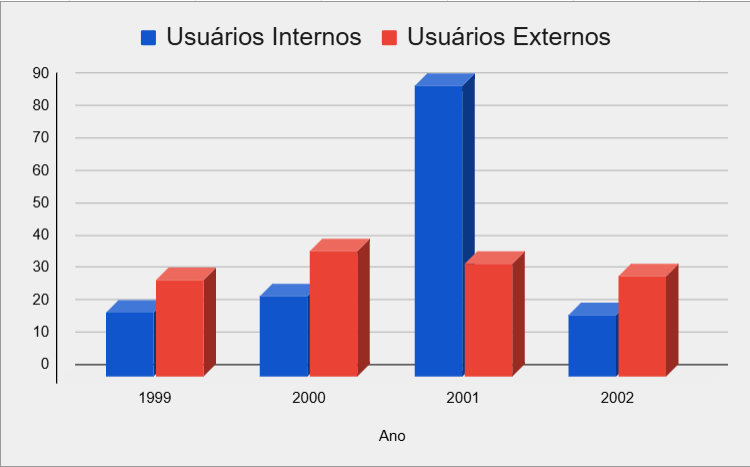
\includegraphics[width=12.5cm,height=7.2cm]{figuras/grafico-tcc.png}
      \legend{Fonte: Silva, Camargo Pires (2004, p. 45)}
      \label{fig:internet}
    \end{figure}

    \clearpage

  \section{Exemplos de Citações}

    {\centering\bfseries\color{red} Exemplos de Citações \par}

    {\centering\bfseries\color{red} Citação direta: \par}

    \bigskip

    Citações diretas de até 3 linhas, devem iniciar e terminar por aspas duplas.

    Se o texto original já contiver aspas duplas, substituí-las por aspas simples. A indicação da fonte da citação pode estar inserida no texto ou após a citação.

    \bigskip

    {\color{red} Exemplo:}

    \bigskip

    Segundo Castro (2001, p. 23): ``Os deveres da conduta do anestesiologista constituem predicados importantes quando se quer avaliar a qualidade do procedimento.''

    %% Note que em latex o abre aspas é a 'crase' dupla e o fecha aspas o 'plic' duplo.

    \bigskip

    {\color{red} ou}

    \bigskip

    ``A expressão 'furiosa' dessa estátua de que fala Rebelais, corresponde também à realidade.'' (BAKHTIN, 1987, p. 89).

    \bigskip

    {\centering\bfseries\color{red} Citação Direta com mais de três linhas: \par}

    \bigskip

    As citações diretas, no texto, com mais de três linhas, devem ser destacadas com recuo de 4 cm da margem esquerda, com letra menor que a do texto utilizado e sem as aspas. A indicação da fonte da citação pode estar inserida no texto ou após a citação.

    \bigskip

    {\color{red} Exemplo:}
    \bigskip
    Sobre mercado financeiro, Fortuna (1996, p. 15) considera:
    \bigskip

    \begin{citacao}
      O mercado financeiro permite que um agente econômico qualquer, sem perspectivas de aplicação, em algum empreendimento próprio, da poupança que é capaz de gerar, seja colocado em contato com outro, cujas perspectivas de investimento superam as respectivas disponibilidades de poupança.
    \end{citacao}

    \bigskip
    A seguir uma citação em inglês:

    \begin{citacao}[english]
      This text is an example in English language in italic with correct hyphenation. This text is an example in English language in italic with correct hyphenation. This text is an example in English language in italic with correct hyphenation.
    \end{citacao}
    \bigskip

    \clearpage{\centering\bfseries\color{red} Citação Indireta: \par}

    \bigskip
    Não se utilizam aspas para esse tipo de citação, nem a(s) página(s) de onde foi extraída a ideia.

    \bigskip
    {\color{red} Exemplo:}
    \bigskip

    A bíblia começou a ser escrita no ano 1.000 a.C. e foi finalizada em 100 d.C., com a morte do último apóstolo, São João, levando aproximadamente 1.150 anos para ser concluída \cite{book:GHELLER}.

    \bigskip
    {\color{red} Exemplo de artigo em anais de evento:}
    \bigskip

    O SOX foi um dos primeiros sistemas operacionais desenvolvidos no Brasil. \cite{Sox2012}.

    \bigskip

    {\color{red} Exemplo de tese de mestrado:}

    \bigskip

    A primeira grande iniciativa de desenvolvimento de software no NCE/UFRJ foi o Sistema COPPE-FORTRAN, mais conhecido como COPPEFOR \cite{Salenbauch72}.

    \bigskip
    {\color{red} Exemplo de tese de doutorado:}

    \bigskip
    O Mulplix foi um dos primeiros sistemas operacionais desenvolvidos no NCE/UFRJ na década de 1990 \cite{Azevedo93}.

    \bigskip

    {\centering\bfseries\color{red} Citação de Citação: \par}

    \bigskip

    A indicação da fonte é feita pelo sobrenome do autor da obra citada (não consultada), ano, seguido da expressão latina apud. Após, indica-se o sobrenome do autor da obra consultada, seguido do ano de publicação, precedido por vírgula. Quando for citação direta incluir a(s) página(s) após a data de publicação, precedida de vírgula.

    \bigskip

    {\sffamily \textrm{\textcolor{red}{Exemplo no texto}}\textrm{:}}

    \bigskip

    {\sffamily \textrm{citado por }}

    \bigskip

    Segundo Marques e Ribeiro \footnote{MARQUES, Alberto; RIBEIRO, \textbf{Angela. As fazendas agrícolas}. São Paulo: Ática, 2000. 350 p.} (2000 apud OLIVEIRA, 2001), \apudonline{art:PRADO}{book:AMADO} o Serviço de Atenção Médico-Sanitário da Suécia tem uma tradição de mais de cem anos.

    \bigskip

    {\color{red} ou}

    \textcolor{red}{Em nota de rodapé}

    \bigskip

    {\centering\bfseries\color{red} Indicação da Citação: \par}

    \bigskip

    {\sffamily \textrm{Se a indicação da fonte da citação estiver incluída na frase, a mesma deve aparecer apenas com a inicial maiúscula seguida de parênteses, com a data de publicação do }\textrm{documento. Quando for citação direta incluir a(s) página(s) após a data de publicação, precedida de vírgula.}}

    \bigskip

    {\color{red} Exemplo com autor pessoal:}

    \bigskip

    Segundo Fonseca(2004, p. 36): ``Se não houver mecanismos jurídicos que assegurem a proteção dos direitos humanos, esse valor não será concretizado pelo Poder Público.''

    \bigskip

    {\sffamily \textrm{\textcolor{red}{Exemplo com dois autores: }}}

    \bigskip

    Tonetto e Reck (2001, p. 134) destacam: ``Este autoconhecimento pressupõe conhecer seus limites [...]''

    \bigskip

    {\color{red} Exemplo com mais de três autores:}

    \bigskip

    Neste contexto, Couto e outros (2004, p. 52) destacam que: ``No capitalismo não é a simples ausência do patrão que promove a superação do despotismo da divisão laboral.''

    \bigskip

    {\sffamily \textrm{\textcolor{red}{Exemplo com autor institucional: }}}

    \bigskip

    De acordo com a Pontifícia Universidade Católica do Rio Grande do Sul (2001, p. 24): ``[...] no horizonte 2001/2010, o esforço estratégico da PUCRS será centrado em sete áreas estratégicas [...]''

    \bigskip

    {\color{red} Exemplo sem autor(es), com a entrada pelo título:}

    \bigskip

    Segundo o Guia de clareamento dental (1996, p. 8): ``A causa mais comum do escurecimento dental é o tratamento endodôntico realizado de modo inadequado e sem os cuidados técnicos.''

    \bigskip

    {\color{red} Exemplo sem autor(es), com a entrada pelo título que inicia por artigo:}

    \bigskip

    O movimento social, com o intuito de realizar uma transformação social, é uma das tarefas mais importantes da atualidade (O COOPERATIVISMO..., 2002).

    \bigskip

    As citações a seguir foram colocadas para que as referências aparecessem na bibliografia. Como exemplo temos os livros de Jorge Amado \cite{book:AMADO} \cite{book:AMADO2}, e este autor que desconheço \cite{book:JOHANSSON}, além de \cite{book:ENGEL} e um artigo \cite{art:PRADO}. Notem que é gerado um link hipertexto no documento em PDF.


  
\chapter{Equações, Códigos,  Remissões e Glossário}\label{chp:capitulo4}

  \section{Equações}\label{sec:equacoes}
    Referência: \url{http://en.wikibooks.org/wiki/LaTeX/Mathematics}

    Também: \url{http://en.wikibooks.org/wiki/LaTeX/Advanced_Mathematics}

    \begin{equation}\label{eq:equacao1}
      (x + y)^2 = x^2 + 2xy + y^2
    \end{equation}

  \section{Códigos}\label{sec:codigos}
    Reference: \url{http://en.wikibooks.org/wiki/LaTeX/Source_Code_Listings}

    %\includecode[Linguagem]{Caption}{Label}{Arquivo}
    \includecode[C]{Exemplo em Linguagem C} {alg:codigo1}{codigos/codigo.c}

    %\includecode[Linguagem]{Caption}{Label}{Arquivo}
    \includecode[Java]{Exemplo em Linguagem Java} {alg:codigo2}{codigos/codigo.java}

  \section{Referências Cruzadas} \label{sec:referencias}

    A seguir como realizar referências cruzadas (remissões) da maneira correta a capítulos, seções, tabelas, etc. que aparecem no texto. Note a primeira letra sempre em caixa alta.

    \begin{itemize}
      \item Capítulo \ref{chp:capitulo4}
      \item Seção \ref{sec:codigos}
      \item Seção \ref{sec:referencias}
      \item Tabela \ref{tab:alimentos}
      \item Quadro \ref{quad:quadro1}
      \item Figura \ref{fig:internet}
      \item Equação \ref{eq:equacao1}
      \item Código \ref{alg:codigo1}
    \end{itemize}

  \section{Glossário}\label{sec:glossario}
    Para produzir um glossário em \Gls{latex} utilize o comando \emph{$\backslash$gls\{termo\}} para incluir a referência a um termo do glossário no texto. Um link de hipertexto será criado automaticamente para o termo no glossário como em \gls{maths}.

    As \glspl{formula} são processadas adequadamente e facilmente uma vez que o usuário se acostuma com os comandos.

    Dado um conjunto de números, há métodos elementares para calcular o seu \acrlong{mdc}, que é abreviado \acrshort{mdc}. Este processo é similar ao utilizado para o  \acrfull{mmc}.

    Veja o arquivo glossario.tex em anexo para alguns exemplos simples.


  
\chapter{CONCLUSÃO}

Onde se expõe o fechamento das ideias do estudo, são apresentados os resultados da pesquisa, e partindo da análise destes resultados, tiram-se as conclusões e se for necessário, as sugestões relativas aos estudos futuros.

Observação: É opcional a apresentação dos desdobramentos relativos à importância, síntese, projeção, repercussão, encaminhamento e outros.


  \postextual

  % Referências (obrigatório)
  \bibliography{elementos-postextuais/referencias.bib}

  % Glossário (opcional)
  \clearpage
  \addcontentsline{toc}{chapter}{GLOSSÁRIO}
  \printglossary

  % Apêndices (opcional)
  % O apêndice é elaborado pelo próprio autor do trabalho e
  % serve para complementar a sua argumentação.
  \clearpage
  \begin{apendicesenv}
    \newpage
    {\let\clearpage\relax \chapter{\textbf{Análise dos
relatórios mensais de uso do serviço de renovação de empréstimos}}}

Quanto aos elementos pós-textuais de um trabalho acadêmico, os apêndices e anexos também se distinguem pela origem do conteúdo. Os \textbf{apêndices} contêm materiais elaborados pelo próprio autor do trabalho, como questionários, entrevistas ou análises complementares, e servem para aprofundar ou esclarecer pontos abordados no texto. Já os anexos reúnem documentos produzidos por terceiros, como leis, mapas, artigos ou imagens, que são incluídos para comprovar ou ilustrar informações discutidas no corpo do trabalho. Ambos devem ser identificados com letras maiúsculas (Apêndice A, Anexo A, etc.), seguidos de um título explicativo (ex: Apêndice A - Questionário aplicado),
 e são inseridos após as referências, \textbf{com os apêndices vindo antes dos anexos}.\\
    \newpage
    {\let\clearpage\relax \chapter[Análise dos relatórios mensais de uso do serviço de emprésti\-mo domiciliar]{\textbf{Análise dos relatórios mensais de uso do serviço de empréstimo domiciliar}}}

Lorem ipsum dolor sit amet, consectetur adipiscing elit. Donec lacus nisl, ultricies vitae semper eu, scelerisque nec enim. Curabitur posuere tortor orci, at porta leo laoreet et. Quisque ut congue dolor. Maecenas vel sagittis diam. Praesent fermentum eleifend mi, sit amet vehicula leo pellentesque quis. Curabitur mattis luctus pulvinar. Proin auctor est nec nulla pellentesque commodo. Donec nec justo eu magna aliquet eleifend. Curabitur tristique tortor id sem dignissim, a iaculis metus interdum. Phasellus bibendum velit sit amet interdum semper. Nam vestibulum dui quis nisi consectetur, id vehicula dolor faucibus.

  \end{apendicesenv}

  % Anexos (opcional)
  % Anexos são é constituídos por documentos complementares ao
  % texto do trabalho e que não são elaborados pelo autor do
  % mesmo, servem para fundamentação, comprovação e ilustração.
  \clearpage
  \begin{anexosenv}
    \newpage
    {\let\clearpage\relax \chapter{\textbf{Demonstrativo de frequência diária ago./set. 2001}}}

Quanto aos elementos pós-textuais de um trabalho acadêmico, os apêndices e anexos também se distinguem pela origem do conteúdo. Os apêndices contêm materiais elaborados pelo próprio autor do trabalho, como questionários, entrevistas ou análises complementares, e servem para aprofundar ou esclarecer pontos abordados no texto. Já os \textbf{anexos} reúnem documentos produzidos por terceiros, como leis, mapas, artigos ou imagens, que são incluídos para comprovar ou ilustrar informações discutidas no corpo do trabalho. Ambos devem ser identificados com letras maiúsculas (Apêndice A, Anexo A, etc.), seguidos de um título explicativo (ex: Apêndice A - Questionário aplicado), e são inseridos após as referências, \textbf{com os apêndices vindo antes dos anexos}.

    \newpage
    {\let\clearpage\relax \chapter{\textbf{Demonstrativo de frequência diária jan./dez. 2002}}}

Lorem ipsum dolor sit amet, consectetur adipiscing elit. Donec lacus nisl, ultricies vitae semper eu, scelerisque nec enim. Curabitur posuere tortor orci, at porta leo laoreet et. Quisque ut congue dolor. Maecenas vel sagittis diam. Praesent fermentum eleifend mi, sit amet vehicula leo pellentesque quis. Curabitur mattis luctus pulvinar. Proin auctor est nec nulla pellentesque commodo. Donec nec justo eu magna aliquet eleifend. Curabitur tristique tortor id sem dignissim, a iaculis metus interdum. Phasellus bibendum velit sit amet interdum semper. Nam vestibulum dui quis nisi consectetur, id vehicula dolor faucibus.

  \end{anexosenv}

\end{document}
